\documentclass[12pt]{article}
\usepackage[
backend=biber,
style=abnt,
sorting=nyt
]{biblatex}
\usepackage{csquotes}
\addbibresource{bibliografia.bib}
\AtBeginBibliography{\raggedright \footnotesize}
\setlength{\bibitemsep}{\baselineskip}

\usepackage{amsmath} %Para usar símbolos matemáticos

\usepackage[brazil]{babel} %Para usar a linguagem português
\addto\captionsbrazil{
    \renewcommand{\contentsname}{\texorpdfstring{\normalsize SUMÁRIO}{SUMÁRIO}}
    \renewcommand{\listtablename}{\texorpdfstring{\normalsize ÍNDICE DE TABELAS}{ÍNDICE DE TABELAS}}
    \renewcommand{\listfigurename}{\texorpdfstring{\normalsize ÍNDICE DE FIGURAS}{ÍNDICE DE FIGURAS}}
}

\usepackage{subcaption}
\usepackage{float}
\usepackage{graphicx} %Para inserir imagens
\usepackage{geometry} %Para alterar propriedades da página
\geometry{
a4paper,
left=30mm,
top=30mm,
right=20mm,
bottom=20mm
}

\usepackage[hidelinks]{hyperref}

\usepackage{tocloft}
\renewcommand{\cfttoctitlefont}{\hfill}
\renewcommand{\cftaftertoctitle}{\hfill}
\renewcommand{\cftsecfont}{\normalsize\normalfont\bfseries}
\renewcommand{\cftsubsecindent}{0pt}
\renewcommand{\cftsubsecfont}{\normalsize\normalfont}
\renewcommand{\cftsubsubsecindent}{0pt}
\renewcommand{\cftsubsubsecfont}{\normalsize\normalfont\bfseries}
\renewcommand{\cftsecleader}{\cftdotfill{\cftdotsep}}
\renewcommand{\cftlottitlefont}{\hfill} %Centralizar o título da lista de tabelas
\renewcommand{\cftafterlottitle}{\hfill}
\renewcommand{\cfttabpresnum}{Tabela\ } %Adicionar Tabela antes do nome de cada item
\renewcommand{\cfttabaftersnum}{:\ }
\setlength{\cfttabnumwidth}{4.75em}
\renewcommand{\cftdotsep}{1}
\renewcommand{\cftloftitlefont}{\hfill}
\renewcommand{\cftafterloftitle}{\hfill}
\renewcommand{\cftfigpresnum}{Figura\ }
\renewcommand{\cftfigaftersnum}{:\ }
\setlength{\cftfignumwidth}{4.75em}

\usepackage{titlesec}
\titleformat{\section}{\normalsize\bfseries\MakeUppercase}{\thesection}{0.5em}{}
\titleformat{\subsection}{\normalsize\MakeUppercase}{\thesubsection}{0.5em}{}
\titleformat{\subsubsection}{\normalsize\bfseries}{\thesubsubsection}{0.5em}{}

\usepackage{fancyhdr}
\pagestyle{fancy}
\fancyhf{} % Limpa os cabeçalhos e rodapés
\fancyhead[R]{\footnotesize\thepage} % Coloca o número da página no canto superior direito
\fancyfoot[C]{} % Remove qualquer número de página no rodapé
\renewcommand{\headrulewidth}{0pt} % Remove a linha horizontal do cabeçalho
\renewcommand{\footrulewidth}{0pt} % Remove a linha horizontal do rodapé

\usepackage{multicol}
\usepackage{pgfplots}
\pgfplotsset{compat=1.18}
\usepackage[american]{circuitikz}
\usetikzlibrary{external}\tikzexternalize
\usetikzlibrary{positioning}

\usepackage{setspace} %Para alterar o espaçamento das linhas
\setstretch{1.5}

\begin{document}
    \begin{titlepage}
    \begin{center}
        \large
        Universidade Federal do Espírito Santo - UFES\\
        Departamento de Computação e Eletrônica - DCEL\\
        Engenharia de Computação
        
        \vfill
        \textbf{
        Relatório da experiência 01\\
        Resistores\\~\\
        }
        
        Disciplina: Circuitos Elétricos I\\
        Prof. Flávio Duarte Couto Oliveira\\
        
        \vfill
        \begin{flushright}
            Pedro Henrique Alves do Nascimento
        \end{flushright}
        
        \vfill
        Espírito Santo\\
        Dezembro 2024
    \end{center}
    \newpage
\end{titlepage}
    
    \listoftables
    \thispagestyle{empty}
    \newpage

    \listoffigures
    \thispagestyle{empty}
    \newpage

    \tableofcontents
    \thispagestyle{empty}
    \newpage

    \section*{Pedro Henrique Alves do Nascimento}
    \section{INTRODUÇÃO TEÓRICA}
    \subsection{LEI DE OHM}\indent
    
    A lei de Ohm é a relação algébrica entre corrente tensão para um resistor \parencite{nilsson}, dada pela Equação \ref{lei-de-ohm}
    \begin{equation}
        V=R\times i \label{lei-de-ohm}
    \end{equation}
    onde $V$ é a tensão, em Volts (V) nos terminais do resistor, $R$ é a resistência elétrica do resistor, em Ohms ($\Omega$) e $i$ a corrente que passa pelo resistor, em Ampères (A).

    Ou seja, traçando-se um gráfico de tensão $\times$ corrente para um resistor ôhmico, tem-se uma função linear, onde $\tan{\alpha}=\frac{V'}{i'}$ é a resistência $R$ daquele resistor, como mostrado na Figura \ref{fig:resistorohmico}.
        \begin{figure}[h!]
            \centering
            \caption{Gráfico $V\times i$ de um resistor ôhmico.}
            \begin{minipage}{0.5\textwidth}
                \centering
                \begin{tikzpicture}
                    \begin{axis}[
                        axis lines=middle,
                        xlabel={$i$},
                        ylabel={$V$},
                        xmin=-0.5, xmax=3,
                        ymin=-0.5, ymax=3,
                        xtick={1.15},
                        xticklabel={$i'$},
                        ytick={2},
                        yticklabel={$V'$}
                    ]
                    \addplot[
                        thick,
                        domain=0:2,
                        samples=5,
                    ] {sqrt(3)*x};
                    \draw[smooth, thick] (0.5,0) arc (0:60:0.5) node[midway] {$\alpha$};
                    \node at (axis cs:0,0) [anchor=north east] {$0$};
                    \draw[dashed, color=gray!50] (0,2) -- (1.15,2) -- (1.15,0);
                    \end{axis}
                \end{tikzpicture}

                \raggedright \footnotesize Fonte: Elaborado pelo autor.
                \label{fig:resistorohmico}
            \end{minipage}
        \end{figure}
    
    \subsection{RESISTORES}\indent

    Resistores são componentes eletrônicos fundamentais, projetados para limitar o fluxo de corrente elétrica em um circuito, convertendo parte dessa energia em calor. Estes dispositivos são tipicamente feitos de materiais com alta resistividade, como carbono ou filme metálico. Dependendo de suas propriedades, os resistores podem ser classificados em fixos, cuja resistência é constante, e variáveis, cuja resistência pode ser ajustada conforme necessário.

    \subsubsection{Resistores Fixos}\indent

    Os resistores fixos possuem características como valor nominal e tolerância, que são determinadas por uma tabela de cores. Cada cor na tabela corresponde a um valor específico, facilitando a identificação e a seleção do resistor adequado para uma aplicação particular. A Tabela \ref{tab:corResist} e a Figura \ref{fig:resistor} ilustram o processo de codificação por cores e a representação de um resistor com suas faixas.
    
    \begin{figure}[H]
        \centering
        \caption{Resistor e suas faixas.}
        \begin{tikzpicture}[scale=2]
            \draw[thick] (-1,0.5) rectangle (1,-0.5);
            \draw[fill=gray] (-1.5,0.1) rectangle (-1,-0.1); 
            \draw[fill=gray] (1,0.1) rectangle (1.5,-0.1);
            \definecolor{auburn}{rgb}{0.43, 0.21, 0.1}
            \draw[fill=auburn] (-0.8,0.5) rectangle (-0.6,-0.5);
            \draw[fill=black] (-0.4,0.5) rectangle (-0.2,-0.5);
            \draw[fill=orange] (0,0.5) rectangle (0.2,-0.5);
            \draw[fill=yellow] (0.6,0.5) rectangle (0.8,-0.5);
            
            \draw[thick, <-] (-0.7,-0.5) -- (-0.7,-1);
            \draw[thick] (-0.7, -1) -- (-1.2,-1) node[left] {1º dígito};
            \draw[thick, <-] (-0.3,-0.5) -- (-0.3,-1.3);
            \draw[thick] (-0.3, -1.3) -- (-1.2,-1.3) node[left] {2º dígito};
            \draw[thick, <-] (0.1,-0.5) -- (0.1,-1.6);
            \draw[thick] (0.1, -1.6) -- (-1.2,-1.6) node[left] {Multiplicador};
            \draw[thick, <-] (0.7,-0.5) -- (0.7,-1.9);
            \draw[thick] (0.7, -1.9) -- (-1.2,-1.9) node[left] {Tolerância};
            \draw (-2.55, -2.2) node[right] {\footnotesize{Fonte: Elaborado pelo autor.}};
        \end{tikzpicture}
        \label{fig:resistor}
    \end{figure}

    \begin{table}[H]
        \caption{Tabela do cores dos resistores fixos.}
        \label{tab:corResist}
        \centering
        % \vspace{0.5em}
        \setstretch{1.5}{
        \begin{tabular}{ccclc}
        \hline
        Cor & 1ª Faixa & 2ª Faixa & Multiplicador ($\Omega$) & Tolerância\\
        \hline Preto & 0 & 0 & $\times 1$ & \\
        Marrom & 1 & 1 & $\times 10$ & $\pm$ 1\%\\
        Vermelho & 2 & 2 & $\times 100$ & $\pm$ 2\%\\
        Laranja & 3 & 3 & $\times 1$ k & \\
        Amarelo & 4 & 4 & $\times 10$ k & \\
        Verde & 5 & 5 & $\times 100$ k & $\pm$ 0.5\%\\
        Azul & 6 & 6 & $\times 1$ M & $\pm$ 0.25\%\\
        Violeta & 7 & 7 & $\times 10$ M & $\pm$ 0.1\%\\
        Cinza & 8 & 8 & & $\pm$ 0.05\%\\
        Branco & 9 & 9 & & \\
        Dourado & & & $\times 0.1$ & $\pm$ 5\%\\
        Prateado & & & $\times 0.01$ & $\pm$ 10\%\\
        \hline
        \end{tabular}}\\
        \footnotesize Fonte: blog.fazedores.com (Adaptado)\nocite{codigo_cores_resistores}.
    \end{table}

    \subsubsection{Resistores Variáveis}\indent

    Os resistores variáveis, como os potenciômetros, são componentes com três terminais. A resistência é ajustada movendo o terminal central em relação aos terminais externos. A resistência máxima é obtida quando o terminal central é posicionado na posição 3 da Figura \ref{fig:potenciometro}.
    
    O funcionamento desses resistores se baseia na variação do comprimento do segmento resistivo. De acordo com a equação $R = \rho\times\frac{L}{A}$ --- onde $R$ é a resistência do material, $\rho$ a sua resistividade, $L$ o comprimento e $A$ a área da seção transversal --- a resistência é diretamente proporcional ao comprimento do resistor.
    
    Assim, quanto mais próximo o terminal central estiver da posição 3, maior será a resistência. A Figura \ref{fig:potenciometro} exemplifica o uso de um potenciômetro em sua representação gráfica.

    Resistores variáveis são amplamente utilizados em dispositivos como controles de volume em equipamentos de áudio, nos quais a resistência ajusta a tensão, afetando diretamente a saída do som.

    \begin{figure}[H]
        \centering
        \caption{Representação gráfica de potenciômetro.}
        \begin{minipage}{0.4\textwidth}
            \centering
            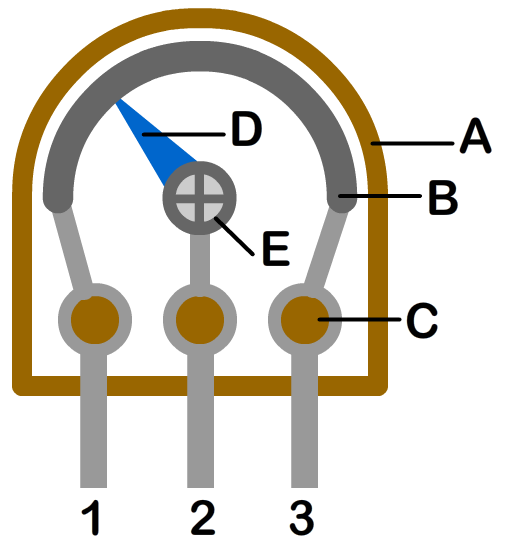
\includegraphics[width=\textwidth]{external-figures/resistor-variavel.png}
            \raggedright \footnotesize Fonte: ricardoteix.com (2021)\nocite{ricardo_teix}.
            \label{fig:potenciometro}
        \end{minipage}
    \end{figure}

    \begin{figure}[H]
        \centering
        \caption{Representação de resistor fixo e variável em um circuito.}
        \begin{tikzpicture}
            \draw (-0.5,0) -- (0,0) to [R, label=$R$] (1,0) -- (1.5,0) to
            [open] (2.5,0) -- (3,0) to
            [vR, l=$R_{var}$] (4,0) -- (4.5,0);
        \end{tikzpicture}
    \end{figure}
    
    \subsection{OHMÍMETRO}\indent

    O ohmímetro é um dispositivo para a medição da resistência elétrica. Para realizar a medição, o ohmímetro deve ser conectado em paralelo com o resistor e não deve ser exposto a nenhuma tensão externa, pois o aparelho funciona fornecendo uma corrente ao resistor e medindo a tensão entre seus terminais \parencite{ohmmeter_website}.
    
    A partir dessa medição, é possível calcular a resistência utilizando a Lei de Ohm. Caso haja uma fonte de tensão adicional no circuito, a medição poderá ser afetada, uma vez que a tensão nos terminais do resistor será influenciada pela presença dessa fonte. A Figura \ref{fig:ohmimetro} ilustra o esquema de ligação do ohmímetro.
    \begin{figure}[H]
        \centering
        \caption{Esquema de ligação de um ohmímetro.}
        \begin{minipage}{0.5\textwidth}
            \centering
            \begin{tikzpicture}
                \draw (-0.5,0) -- (0,0) to [R, l=$R$] (3,0) to
                [short, *-] (3,2) to
                [rmeterwa, t=$\Omega$] (0,2) to
                [short, -*] (0,0);
                \draw (3,0) -- (3.5,0);
            \end{tikzpicture}
            \label{fig:ohmimetro}
        \end{minipage}
    \end{figure}

\section{PRÁTICA EM LABORATÓRIO}\indent

Primeiramente, foram identificados 10 resistores com base na cor de cada uma de suas faixas  e anotou-se seus valores nominais e tolerâncias.

Após isso, mediu-se a resistência de cada resistor com um multímetro na escala de resistência e anotou-se os valores medidos. Então, calculou-se o erro utilizando a Equação \ref{eq:erro}:
\begin{equation}
    Erro(\%) = \left(1 - \frac{R_{medido}}{R_{nominal}}\right)\times 100\%
    \label{eq:erro}
\end{equation}

Os resultados medidos estão contidos na Tabela \ref{tab:erro_resistores}.
\begin{table}[H]
    \caption{Valores e nominais e erro de medição dos resistores.}
    \label{tab:erro_resistores}
    \centering
    \setstretch{1.5}{
    \begin{tabular}{ccccc}
        \hline Resistor & Valor nominal ($\Omega$) & Tolerância (\%) & Valor medido ($\Omega$) & Erro (\%)\\
        \hline $R_1$ & & & & \\
        $R_2$ & & & & \\
        $R_3$ & & & & \\
        $R_4$ & & & & \\
        $R_5$ & & & & \\
        $R_6$ & & & & \\
        $R_7$ & & & & \\
        $R_8$ & & & & \\
        $R_9$ & & & & \\
        $R_{10}$ & & & & \\
        \hline
    \end{tabular}}


    \footnotesize{Fonte: Elaborado pelo autor.}
\end{table}

\begin{center}\small
    \begin{circuitikz}[american]
        \draw (0,0) to [resistor, l=10 $\Omega$] (3,0) to [short, *-] (3,0)
        to [resistor, l_=60 $\Omega$] (3,2)
        to [resistor, l_=10 $\Omega$] (3,4)
        to [resistor, l_=130 $\Omega$] (3,6)
        to [short, *-, f_<=$i_g$] (0,6)
        to [voltage source, v_=600 V, sources/scale=2] (0,0);
        \draw (3,6) to [R, l=34 $\Omega$] (7,6)
        to [short, *-] (7,6)
        to [R, l=72 $\Omega$, f_=$i_0$] (7,3)
        to [R, l=8 $\Omega$] (7,0)
        to [short, -*] (7,0)
        to (7,0) -- (3,0);
        \draw (7,6) to (7,6) -- (10,6)
        to [R, l=20 $\Omega$] (10,0)
        to (10,0) -- (7,0);
    \end{circuitikz}
\end{center}

\begin{center}
\Large
\begin{circuitikz}[scale=0.5, transform shape]
    \node (A) at (6.5,3) {};
    \node (B) at (8.5,3) {};
    \ctikzset{nodes width=0.08};
    \draw(0,0) to [short, -*] (3,0)
    to [R, l_=3 k$\Omega$, -*] (3,3)
    to [R, l_=2 k$\Omega$, -*] (3,6)
    to [short] (0,6)
    to [current source, l_=4.5 mA, invert, sources/scale=2] (0,0);
    \draw (3,6) to [short] (12,6)
    to [R, l=1.5 k$\Omega$, -*] (12,3)
    to [R, l=6 k$\Omega$] (12,0)
    to [short] (3,0);
    \draw (3,3) to [R, l=1 k$\Omega$, -*] (A) node[label={above: +}] {};
    \draw (12,3) to [R, l_=5 k$\Omega$, -*] (B) node[label={above: -}] {};
    \draw (A) to [open, l=$v_0$] (B);
\end{circuitikz}
\end{center} 

\newpage
\setstretch{1}
\section*{\hfill REFERÊNCIAS BIBLIOGRÁFICAS\hfill}
\addcontentsline{toc}{section}{REFERÊNCIAS BIBLIOGRÁFICAS}
\printbibliography[heading=none]
\end{document}